\section {Appendix}
\subsection{Logistic Regression on Behavior Data}

\begin{figure}[H] 
\centering 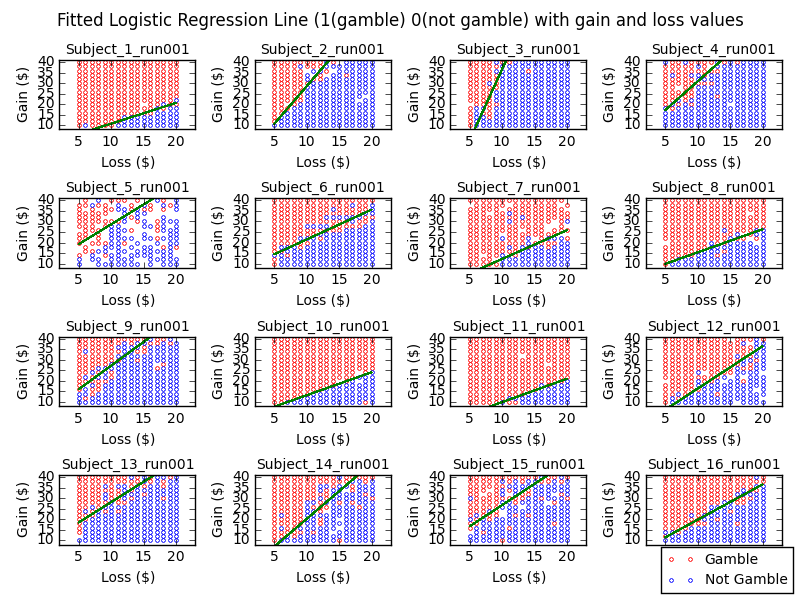
\includegraphics[scale=0.5]{../fig/log_reg_behav/log_regression_behav_subplots.png}	 
\caption{Logistic Regression on each subjects’ behavior data}
\end{figure} 

\subsection{Choosing the more accruate convolved predictor}
\begin{figure}[H] 
\centering 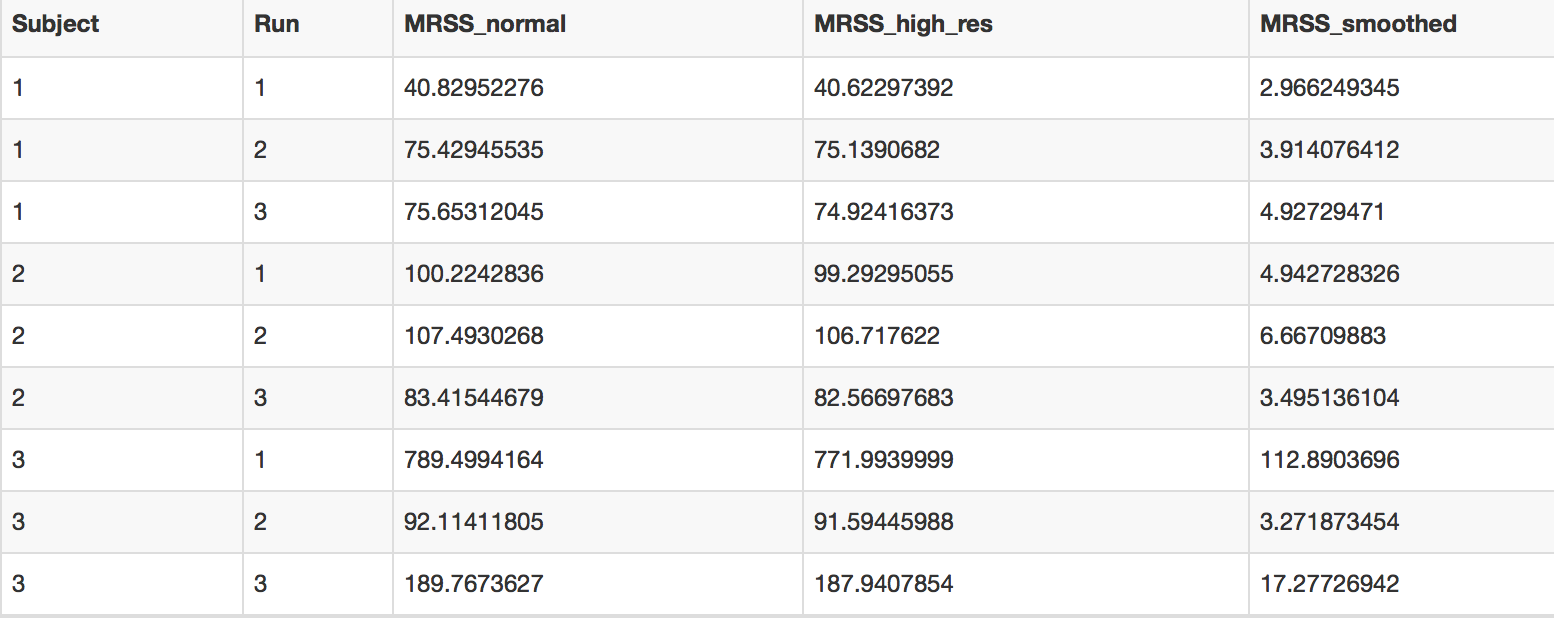
\includegraphics[scale=0.35]{../fig/mrss_result/mrss_result.png}   
\caption{MRSS comparison table}
\end{figure} 

\subsection{Multi-comparison across 16 subjects on TASK condition}
\begin{figure}[H] 
\centering 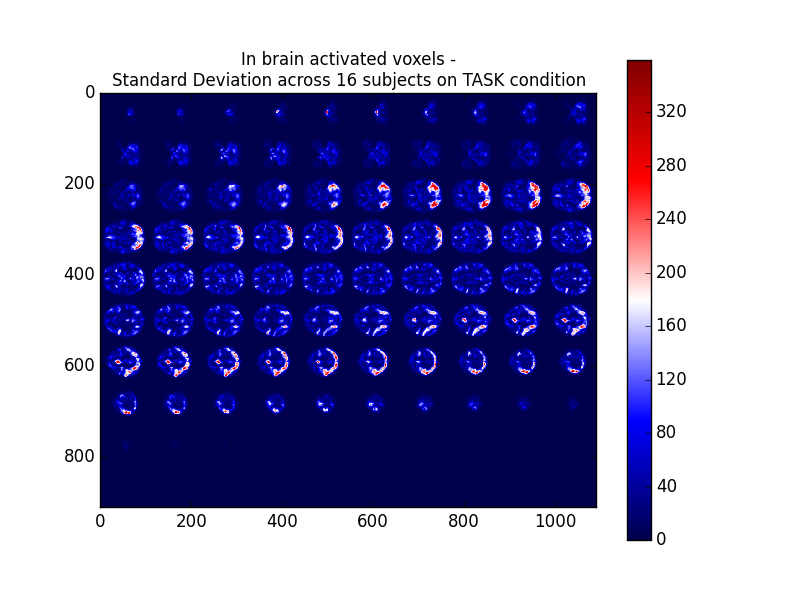
\includegraphics[scale=0.5]{../fig/multi_beta/std_task.png}	 
\caption{Standard Deviation of beta values on each voxel across 16 subjects on TASK condition}
\end{figure} 

\begin{figure}[H] 
\centering 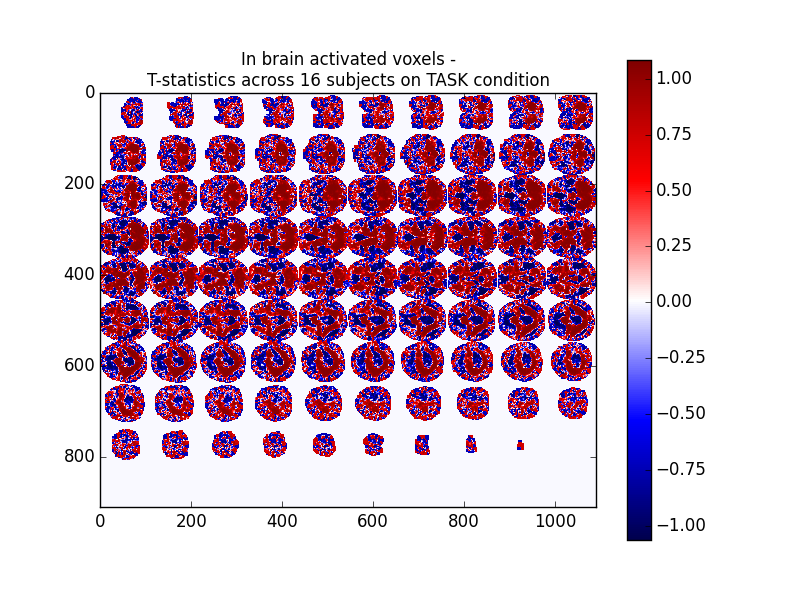
\includegraphics[scale=0.5]{../fig/multi_beta/tstat_task.png}	 
\caption{T-statistics of beta values on each voxel across 16 subjects on TASK condition}
\end{figure} 

\begin{figure}[H] 
\centering 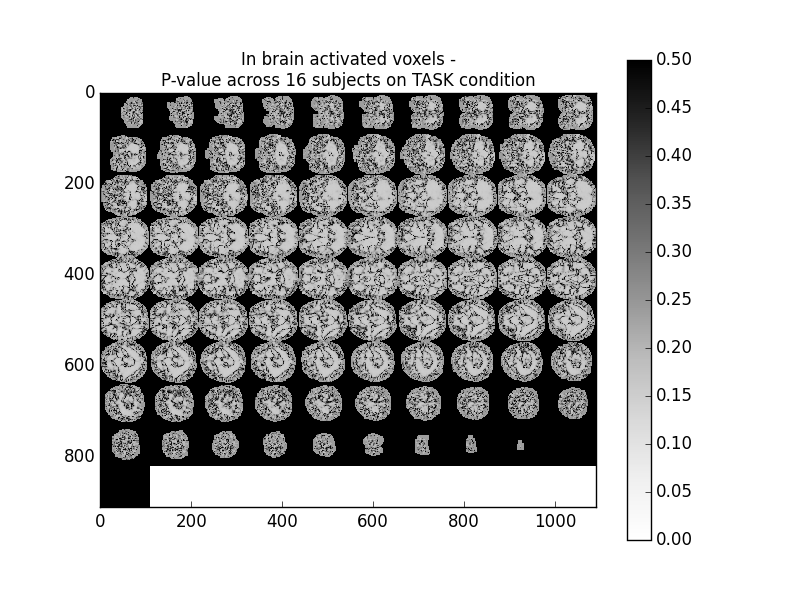
\includegraphics[scale=0.5]{../fig/multi_beta/pval_task.png}	 
\caption{P-value of on each voxel across 16 subjects on TASK condition}
\end{figure} 

\begin{center}
Example 1: Multi-comparison across subjects on TASK condition. P-value indicates the porton of activated
voxels
\end{center}

\subsection{Brain activation for design matrix including drifts terms}
\begin{figure}[H]
\begin{subfigure}{.5\textwidth}
  \centering
  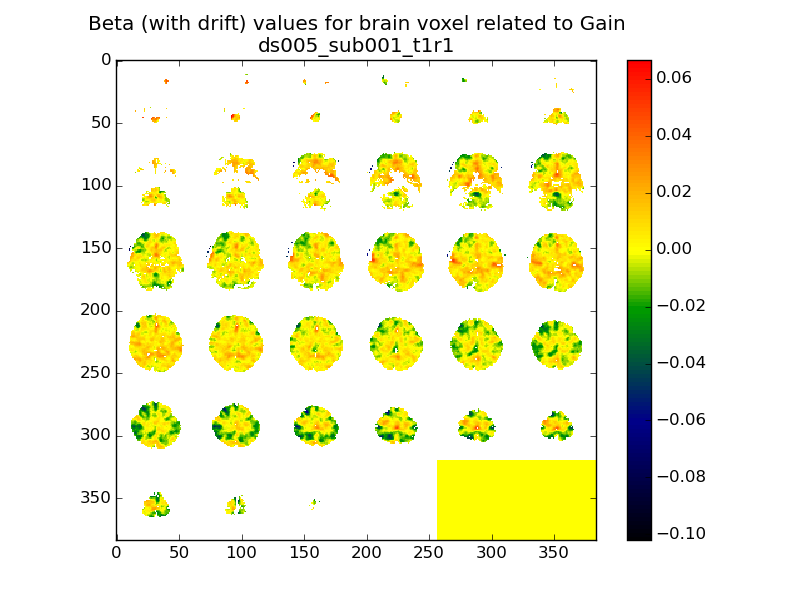
\includegraphics[width=.9\linewidth]{../fig/mosaic/ds005_sub001_t1r1_withdrift_Gain.png}
  \caption{Gain}
  \label{fig:sfig1}
\end{subfigure}%
\begin{subfigure}{.5\textwidth}
  \centering
  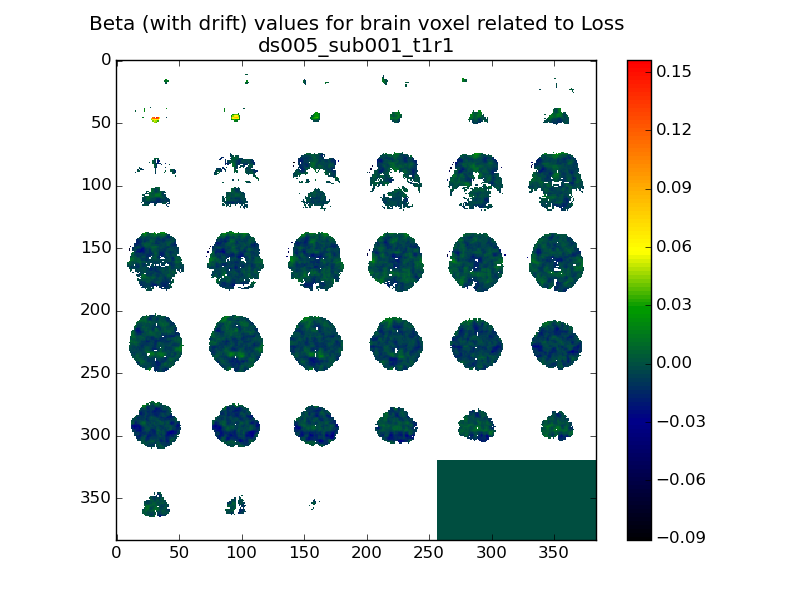
\includegraphics[width=.9\linewidth]{../fig/mosaic/ds005_sub001_t1r1_withdrift_Loss.png}
  \caption{Loss}
  \label{fig:sfig2}
\end{subfigure}
\caption{Betas values of the voxels associated to Gain and Loss - subject 1 run 1}
\label{fig:fig}
\end{figure}

\begin{figure}[H]
\begin{subfigure}{.5\textwidth}
  \centering
  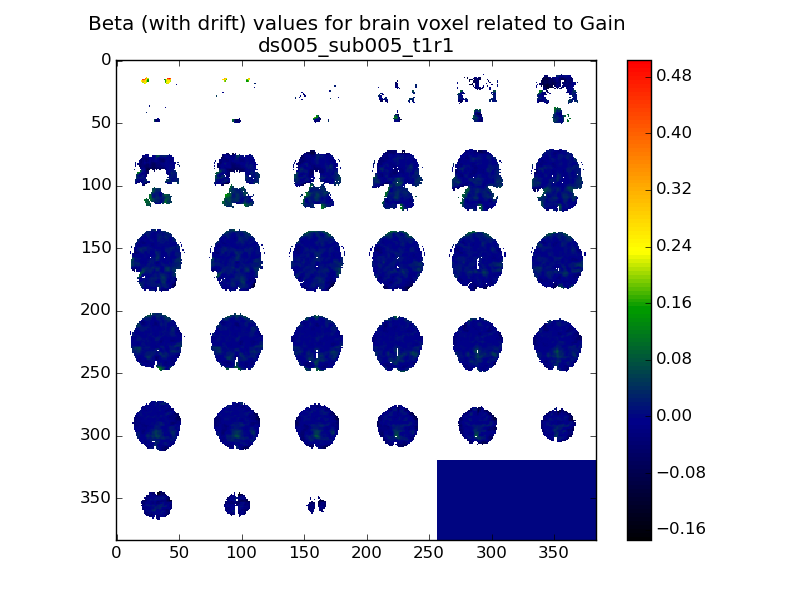
\includegraphics[width=.9\linewidth]{../fig/mosaic/ds005_sub005_t1r1_withdrift_Gain.png}
  \caption{Gain}
  \label{fig:fig1}
\end{subfigure}%
\begin{subfigure}{.5\textwidth}
  \centering
  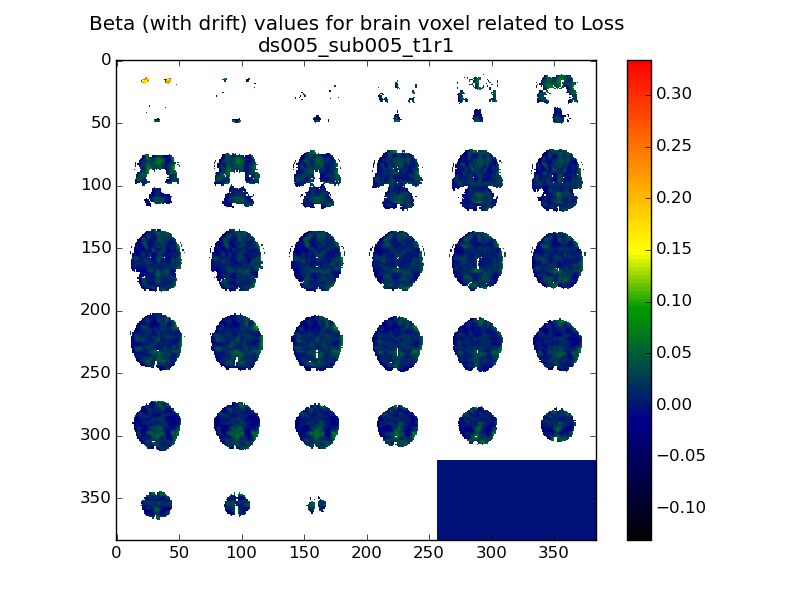
\includegraphics[width=.9\linewidth]{../fig/mosaic/ds005_sub005_t1r1_withdrift_Loss.png}
  \caption{Loss}
  \label{fig:fig2}
\end{subfigure}
\caption{Betas values of the voxels associated to Gain and Loss - subject 5 run 1}
\label{fig:figa}
\end{figure}


\begin{figure}[H]
\begin{subfigure}{.5\textwidth}
  \centering
  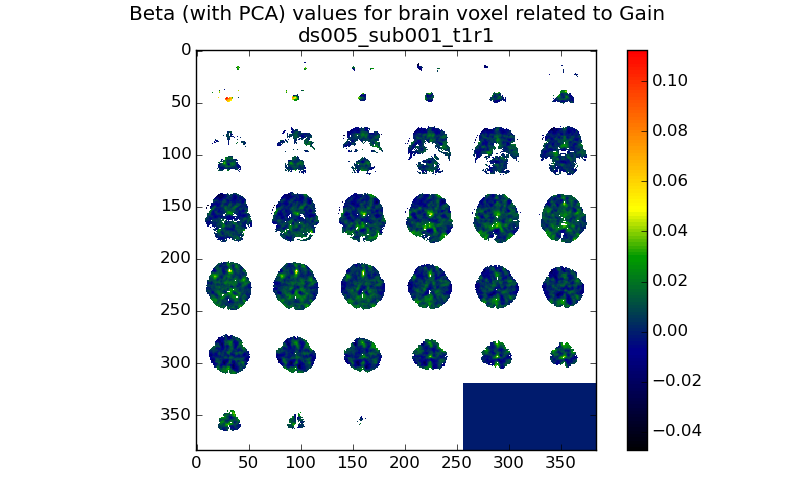
\includegraphics[width=.95\linewidth]{../fig/mosaic/ds005_sub001_t1r1_withPCA_Gain.png}
  \caption{Gain}
  \label{fig:sfig1}
\end{subfigure}%
\begin{subfigure}{.5\textwidth}
  \centering
  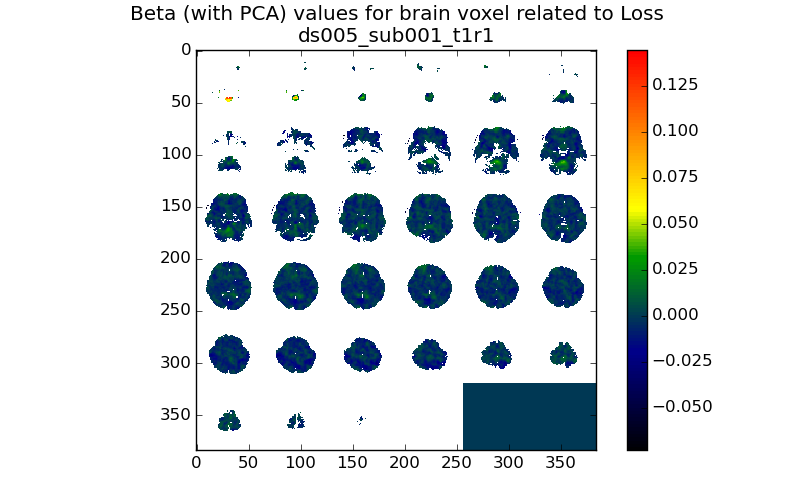
\includegraphics[width=.95\linewidth]{../fig/mosaic/ds005_sub001_t1r1_withPCA_Loss.png}
  \caption{Loss}
  \label{fig:sfig2}
\end{subfigure}
\caption{Betas values of the voxels associated to Gain and Loss - subject 1 run 1}
\label{fig:fig}
\end{figure}

\begin{figure}[H]
\begin{subfigure}{.5\textwidth}
  \centering
  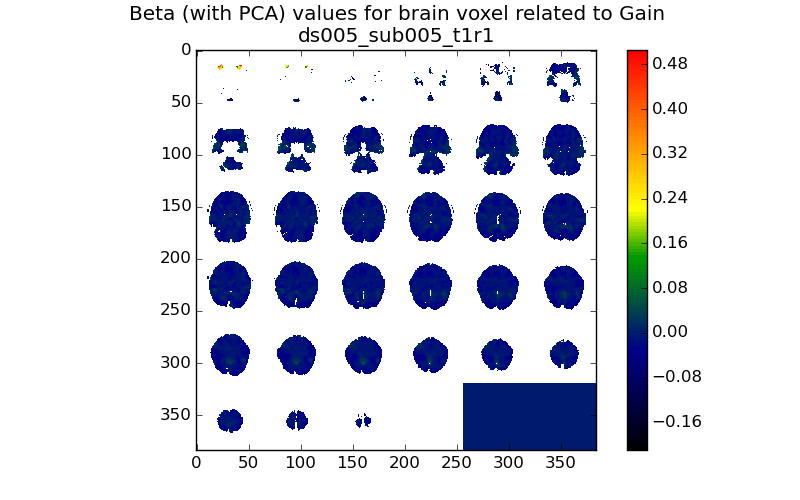
\includegraphics[width=.95\linewidth]{../fig/mosaic/ds005_sub005_t1r1_withPCA_Gain.png}
  \caption{Gain}
  \label{fig:fig1}
\end{subfigure}%
\begin{subfigure}{.5\textwidth}
  \centering
  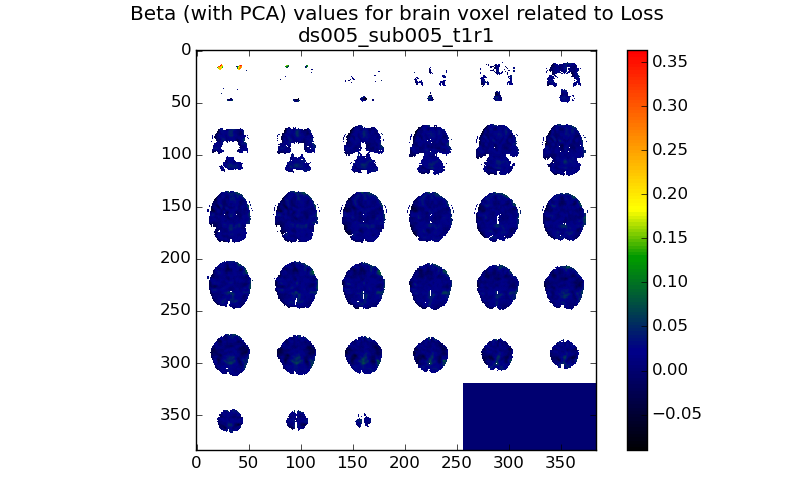
\includegraphics[width=.95\linewidth]{../fig/mosaic/ds005_sub005_t1r1_withPCA_Loss.png}
  \caption{Loss}
  \label{fig:fig2}
\end{subfigure}
\caption{Betas values of the voxels associated to Gain and Loss - subject 5 run 1}
\label{fig:figa}
\end{figure}

\subsection{Some analysis with the filtered data}

\begin{figure}[H]
\begin{subfigure}{.5\textwidth}
  \centering
  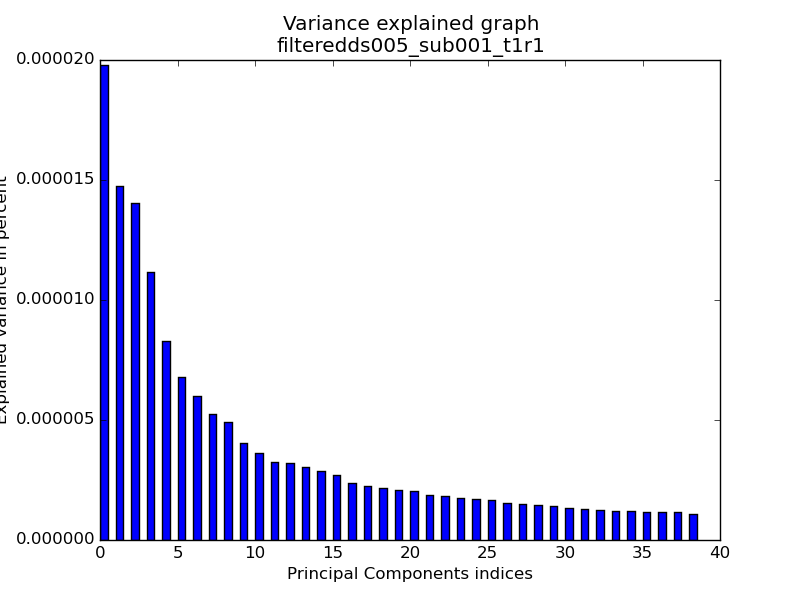
\includegraphics[width=.9\linewidth]{../fig/pca/filteredds005_sub001_t1r1_variance_explained.png}
  \caption{Subject 1}
  \label{fig:fig3}
\end{subfigure}%
\begin{subfigure}{.5\textwidth}
  \centering
  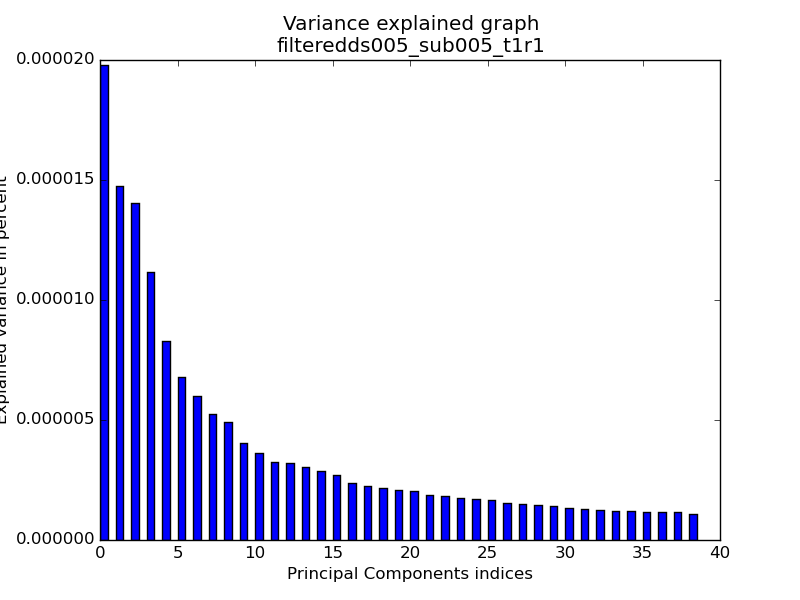
\includegraphics[width=.9\linewidth]{../fig/pca/filteredds005_sub005_t1r1_variance_explained.png}
  \caption{Subject 5}
  \label{fig:fig4}
\end{subfigure}
\caption{Variance explained for filtered data - run 1 for subject 1 and 5}
\label{fig:figb}
\end{figure}


